% !TEX root = ../ClassicThesis.tex
% !TEX spellcheck = en-US

\chapter{Used Hardware and Software or your self-build Prototype}
\label{sec:hw}
Explain the stuff you used. Maybe you have used a special \ac{API} or \ac{UML} for your design process. \ac{UML} is often used in the software architecture design process. If there are very important points in your code you could provide them as listing as seen in \autoref{list:example} or attatch them as appendix.

\section{My Very special Prototype}
Explain your one and only device

\subsection{Device functions}
is it able to roast a chicken while scanning a book for new content?

\subsection{Build Process}
Document the build procedure. Include some photos like  \autoref{fig:example-hw}.

\begin{figure}[bth]
        \myfloatalign
        \subfloat[Asia personas duo.]
        {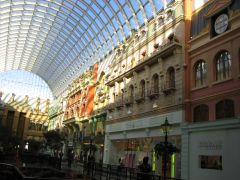
\includegraphics[width=.45\linewidth]{gfx/example_1}} \quad
        \subfloat[Pan ma signo.]
        {\label{fig:example-hw-b}%
         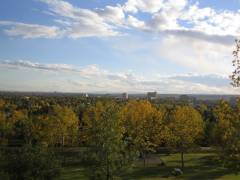
\includegraphics[width=.45\linewidth]{gfx/example_2}} \\
        \subfloat[Methodicamente o uno.]
        {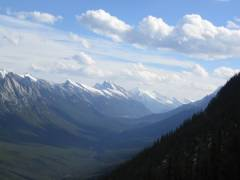
\includegraphics[width=.45\linewidth]{gfx/example_3}} \quad
        \subfloat[Titulo debitas.]
        {
\includegraphics[width=.45\linewidth]{gfx/example_4}}
        \caption[Tu duo titulo debitas latente]{Tu duo titulo debitas
        latente.}\label{fig:example-hw}
\end{figure}


\begin{lstlisting}[frame=lt,caption={Example Listing},label=list:example]
% **************************************************
% 2. Personal data and user ad-hoc commands
% **************************************************
\newcommand{\myTitle}{A Classic Thesis Style\xspace} 
\newcommand{\mySubtitle}{An Homage to...\xspace} 
\caption[Example listing]{Listing Example.}
\label{list:example}
\end{lstlisting}